\documentclass[9pt]{beamer}
\usepackage[utf8]{inputenc}
\usepackage{adjustbox}
\usepackage{amsmath,amssymb,amsthm}
\usepackage{cancel}
\usepackage{float}
\usepackage{mathtools}
\usepackage{tcolorbox}
\usepackage{texdraw}
\usepackage{tikz}
\usepackage{tikz-cd}
\usepackage{todonotes}
\usepackage{blkarray}

\tikzset{
commutative diagrams/.cd,
arrow style=tikz,
diagrams={>=latex}}

\usetheme{Warsaw}

\makeatletter
\setbeamertemplate{footline}
{
    \leavevmode%
    \hbox{%
    \begin{beamercolorbox}[wd=.5\paperwidth,ht=3.5ex,dp=2ex,center]{title in head/foot}%
        \usebeamerfont{name in head/foot}{\footnotesize Recovering Matroids}
    \end{beamercolorbox}%
    \begin{beamercolorbox}[wd=.5\paperwidth,ht=3.5ex,dp=2ex,center]{date in head/foot}%
        \usebeamerfont{name in head/foot}{\footnotesize \insertauthor{}}
    \end{beamercolorbox}}%
    \vskip0pt%
}
\makeatother

\usetikzlibrary{arrows.meta}

\def\calM{\mathcal M}
\def\calC{\mathcal C}
\def\calI{\mathcal I}
\def\calD{\mathcal D}
\def\calB{\mathcal B}
\def\calF{\mathcal F}
\def\calN{\mathcal N}
\def\calP{\mathcal P}
\def\calS{\mathcal S}
\def\calV{\mathcal V}
\def\Z{\mathbb Z}

\title{Constructive Torelli Theorem for Regular Matroids}
\author{Alec Elhindi}
\date{4th November 2024}

\usepackage{graphicx}
\graphicspath{{./images/}}

\newcounter{definition}

\renewcommand{\definition}[1]{\vspace{6pt}\textbf{Definition~\refstepcounter{definition}\thedefinition}: \textit{#1}\vspace{6pt}}

\newcounter{conjecture}

\newcommand{\conjecture}[1]{\vspace{6pt}\textbf{Conjecture~\refstepcounter{conjecture}\theconjecture}: \textit{#1}\vspace{6pt}}

\renewcommand{\theorem}[1]{\vspace{6pt}\textbf{Theorem~\refstepcounter{theorem}\thetheorem}: \textit{#1}\vspace{6pt}}

\renewcommand{\corollary}[1]{\vspace{6pt}\textbf{Corollary}: \textit{#1}\vspace{6pt}}

\newcounter{proposition}

\newcommand{\proposition}[1]{\textbf{Proposition}: #1}

\renewcommand{\example}[1]{\textbf{Example}: #1}

\renewcommand{\proof}[1]{\textbf{Proof}: #1\vspace{12pt}}

\newcommand{\notation}[1]{\textbf{Notation}: #1}

\renewcommand{\qedsymbol}{$\blacksquare$}

\makeatletter
\newcommand{\vast}{\bBigg@{4}}
\newcommand{\Vast}{\bBigg@{5}}
\makeatother

\definecolor{electricpurple}{rgb}{0.75, 0.0, 1.0}

\newcommand{\red}[1]{{\color{red} #1}}
\newcommand{\blue}[1]{{\color{blue} #1}}
\newcommand{\orange}[1]{{\color{orange} #1}}
\newcommand{\purple}[1]{{\color{electricpurple} #1}}

\makeatletter
\let\save@measuring@true\measuring@true
\def\measuring@true{%
  \save@measuring@true
  \def\beamer@sortzero##1{\beamer@ifnextcharospec{\beamer@sortzeroread{##1}}{}}%
  \def\beamer@sortzeroread##1<##2>{}%
  \def\beamer@finalnospec{}%
}
\makeatother

\usetikzlibrary{decorations.markings}

\usetikzlibrary{intersections}

\tikzset{->-/.style={decoration={
    markings,
    mark=at position .5 with {\arrow{>}}},postaction={decorate}}}

\tikzset{-->-/.style={decoration={
    markings,
    mark=at position .75 with {\arrow{>}}},postaction={decorate}}}

\tikzset{->--/.style={decoration={
    markings,
    mark=at position .25 with {\arrow{>}}},postaction={decorate}}}

\tikzcdset{scale cd/.style={every label/.append style={scale=#1},
    cells={nodes={scale=#1}}}}

\DeclarePairedDelimiter\abs{\lvert}{\rvert}

\DeclarePairedDelimiter\norm{\lVert}{\rVert}

\DeclarePairedDelimiter\iprod{\langle}{\rangle}

\begin{document}

    \begin{frame}

        \titlepage

    \end{frame}

    \begin{frame}{Graph Preliminaries}

        A \textbf{graph} $G=(V, E)$ consists of \textbf{vertices} $v_i\in V$ and \textbf{edges} $e_i=\{v_j, v_k\}\in E$.
        
        \begin{center}
        
            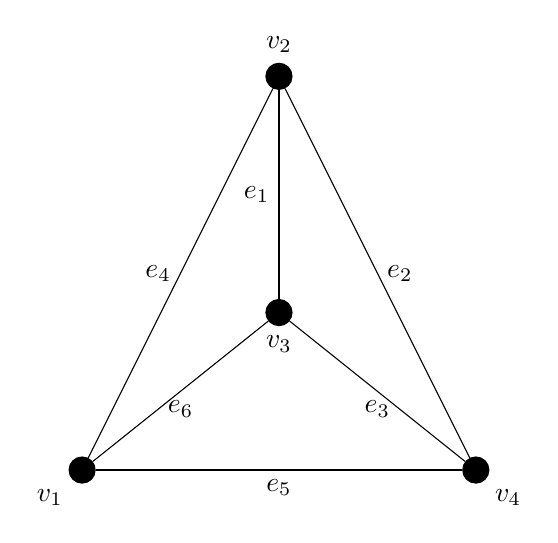
\begin{tikzpicture}
    
                \node[shape=circle, draw=black, fill=black, label=below left:$v_1$] (A) at (-2.5,-2) {};
                \node[shape=circle, draw=black, fill=black, label=above:$v_2$] (B) at (0,3) {};
                \node[shape=circle, draw=black, fill=black, label=below:$v_3$] (C) at (0,0) {};
                \node[shape=circle, draw=black, fill=black, label=below right:$v_4$] (D) at (2.5,-2) {};
            
                \draw (C) -- (B) node[midway, left] {$e_1$};
                \draw (B) -- (D) node[midway, right] {$e_2$};
                \draw (D) -- (C) node[midway, below] {$e_3$};
                \draw (A) -- (B) node[midway, left] {$e_4$};
                \draw (D) -- (A) node[midway, below] {$e_5$};
                \draw (A) -- (C) node[midway, below] {$e_6$};
        
            \end{tikzpicture}
            
        \end{center}

        A\textcolor{white}{n oriented} graph is \textbf{\textcolor{white}{strongly} connected} if there is a\textcolor{white}{n oriented} path between any two vertices.

    \end{frame}

    \begin{frame}{Graph Preliminaries}

        It can be \textbf{oriented}, edges become ordered pairs $e_i=(v_j, v_k)$.
        
        \begin{center}
        
            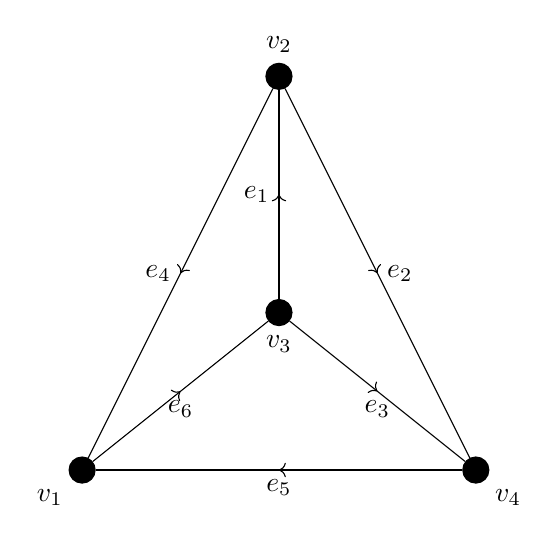
\begin{tikzpicture}
            
                \node[shape=circle, draw=black, fill=black, label=below left:$v_1$] (A) at (-2.5,-2) {};
                \node[shape=circle, draw=black, fill=black, label=above:$v_2$] (B) at (0,3) {};
                \node[shape=circle, draw=black, fill=black, label=below:$v_3$] (C) at (0,0) {};
                \node[shape=circle, draw=black, fill=black, label=below right:$v_4$] (D) at (2.5,-2) {};
            
                \draw[->-] (C) -- (B) node[midway, left] {$e_1$};
                \draw[->-] (B) -- (D) node[midway, right] {$e_2$};
                \draw[->-] (C) -- (D) node[midway, below] {$e_3$};
                \draw[->-] (B) -- (A) node[midway, left] {$e_4$};
                \draw[->-] (D) -- (A) node[midway, below] {$e_5$};
                \draw[->-] (A) -- (C) node[midway, below] {$e_6$};
        
            \end{tikzpicture}
            
        \end{center}

        An oriented graph is \textbf{strongly connected} if there is an oriented path between any two vertices.

    \end{frame}

    \begin{frame}{Connectedness}
        
        A graph is \textbf{$n$-connected} if upon removing $n-1$ edges it remains connected.

        \vspace{12pt}

        A \textbf{cycle} in a graph is a subset $C\subseteq E$ which is a minimal closed walk.

        \vspace{12pt}

        A graph is $2$-connected if every edge participates in a cycle.

    \end{frame}

    \begin{frame}{Cycles}

        \begin{center}
        
            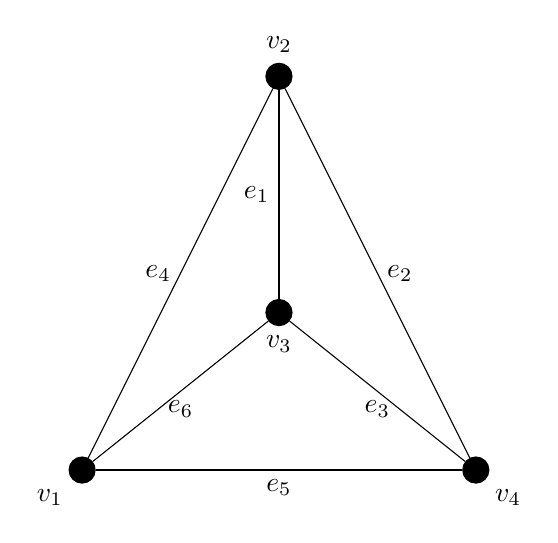
\begin{tikzpicture}
    
                \node[shape=circle, draw=black, fill=black, label=below left:$v_1$] (A) at (-2.5,-2) {};
                \node[shape=circle, draw=black, fill=black, label=above:$v_2$] (B) at (0,3) {};
                \node[shape=circle, draw=black, fill=black, label=below:$v_3$] (C) at (0,0) {};
                \node[shape=circle, draw=black, fill=black, label=below right:$v_4$] (D) at (2.5,-2) {};
            
                \draw (C) -- (B) node[midway, left] {$e_1$};
                \draw (B) -- (D) node[midway, right] {$e_2$};
                \draw (D) -- (C) node[midway, below] {$e_3$};
                \draw (A) -- (B) node[midway, left] {$e_4$};
                \draw (D) -- (A) node[midway, below] {$e_5$};
                \draw (A) -- (C) node[midway, below] {$e_6$};
        
            \end{tikzpicture}
            
        \end{center}

    \end{frame}

    \begin{frame}{Cycles}

        \begin{center}
        
            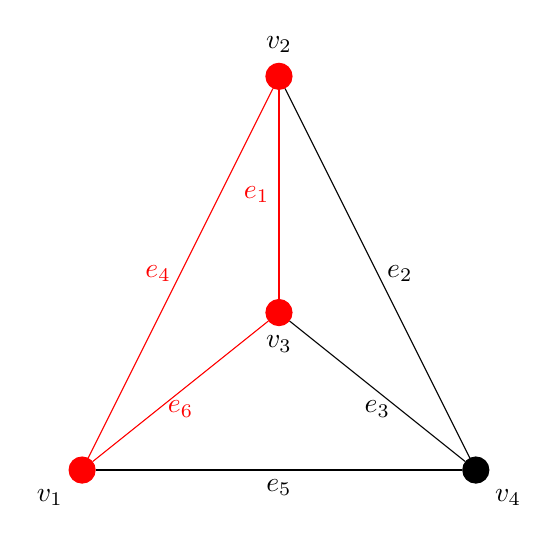
\begin{tikzpicture}
    
                \node[shape=circle, draw=red, fill=red, label=below left:$v_1$] (A) at (-2.5,-2) {};
                \node[shape=circle, draw=red, fill=red, label=above:$v_2$] (B) at (0,3) {};
                \node[shape=circle, draw=red, fill=red, label=below:$v_3$] (C) at (0,0) {};
                \node[shape=circle, draw=black, fill=black, label=below right:$v_4$] (D) at (2.5,-2) {};
            
                \draw[red] (C) -- (B) node[midway, left] {$e_1$};
                \draw (B) -- (D) node[midway, right] {$e_2$};
                \draw (D) -- (C) node[midway, below] {$e_3$};
                \draw[red] (A) -- (B) node[midway, left] {$e_4$};
                \draw (D) -- (A) node[midway, below] {$e_5$};
                \draw[red] (A) -- (C) node[midway, below] {$e_6$};
        
            \end{tikzpicture}
            
        \end{center}

    \end{frame}

    \begin{frame}{Cycles}

        \begin{center}
        
            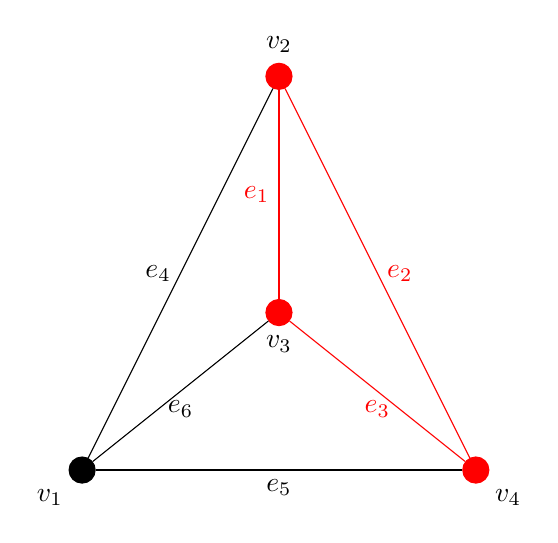
\begin{tikzpicture}
    
                \node[shape=circle, draw=black, fill=black, label=below left:$v_1$] (A) at (-2.5,-2) {};
                \node[shape=circle, draw=red, fill=red, label=above:$v_2$] (B) at (0,3) {};
                \node[shape=circle, draw=red, fill=red, label=below:$v_3$] (C) at (0,0) {};
                \node[shape=circle, draw=red, fill=red, label=below right:$v_4$] (D) at (2.5,-2) {};
            
                \draw[red] (C) -- (B) node[midway, left] {$e_1$};
                \draw[red] (B) -- (D) node[midway, right] {$e_2$};
                \draw[red] (D) -- (C) node[midway, below] {$e_3$};
                \draw (A) -- (B) node[midway, left] {$e_4$};
                \draw (D) -- (A) node[midway, below] {$e_5$};
                \draw (A) -- (C) node[midway, below] {$e_6$};
        
            \end{tikzpicture}
            
        \end{center}

    \end{frame}

    \begin{frame}{Cycles}

        \begin{center}
        
            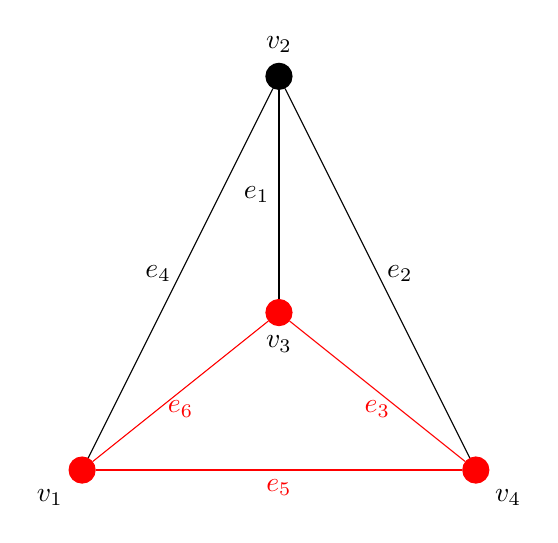
\begin{tikzpicture}
    
                \node[shape=circle, draw=red, fill=red, label=below left:$v_1$] (A) at (-2.5,-2) {};
                \node[shape=circle, draw=black, fill=black, label=above:$v_2$] (B) at (0,3) {};
                \node[shape=circle, draw=red, fill=red, label=below:$v_3$] (C) at (0,0) {};
                \node[shape=circle, draw=red, fill=red, label=below right:$v_4$] (D) at (2.5,-2) {};
            
                \draw (C) -- (B) node[midway, left] {$e_1$};
                \draw (B) -- (D) node[midway, right] {$e_2$};
                \draw[red] (D) -- (C) node[midway, below] {$e_3$};
                \draw (A) -- (B) node[midway, left] {$e_4$};
                \draw[red] (D) -- (A) node[midway, below] {$e_5$};
                \draw[red] (A) -- (C) node[midway, below] {$e_6$};
        
            \end{tikzpicture}
            
        \end{center}

    \end{frame}

    \begin{frame}{Cycles}

        \begin{center}
        
            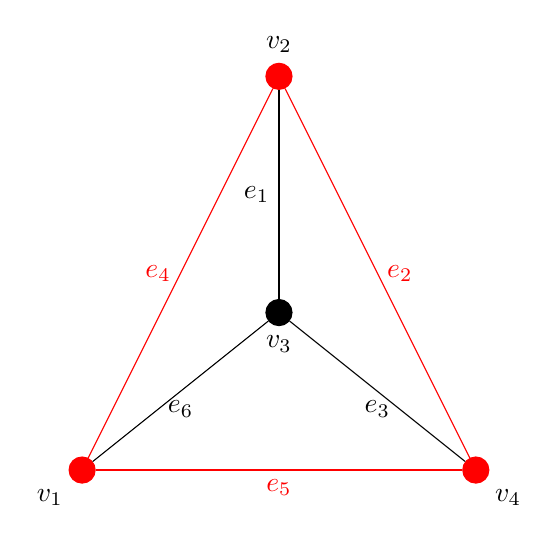
\begin{tikzpicture}
    
                \node[shape=circle, draw=red, fill=red, label=below left:$v_1$] (A) at (-2.5,-2) {};
                \node[shape=circle, draw=red, fill=red, label=above:$v_2$] (B) at (0,3) {};
                \node[shape=circle, draw=black, fill=black, label=below:$v_3$] (C) at (0,0) {};
                \node[shape=circle, draw=red, fill=red, label=below right:$v_4$] (D) at (2.5,-2) {};
            
                \draw (C) -- (B) node[midway, left] {$e_1$};
                \draw[red] (B) -- (D) node[midway, right] {$e_2$};
                \draw (D) -- (C) node[midway, below] {$e_3$};
                \draw[red] (A) -- (B) node[midway, left] {$e_4$};
                \draw[red] (D) -- (A) node[midway, below] {$e_5$};
                \draw (A) -- (C) node[midway, below] {$e_6$};
        
            \end{tikzpicture}
            
        \end{center}

    \end{frame}

    \begin{frame}{Cycles}

        \begin{center}
        
            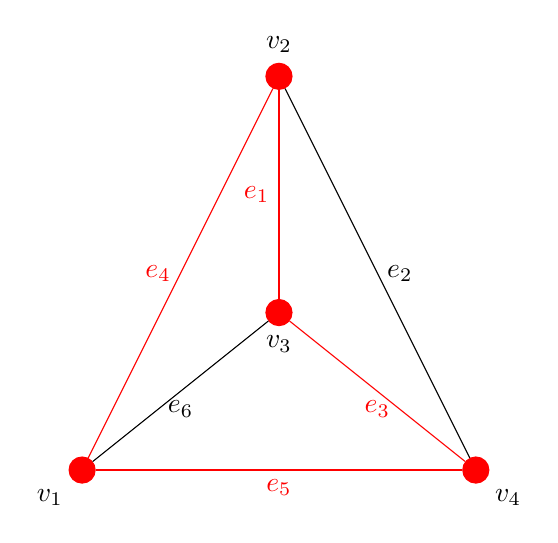
\begin{tikzpicture}
    
                \node[shape=circle, draw=red, fill=red, label=below left:$v_1$] (A) at (-2.5,-2) {};
                \node[shape=circle, draw=red, fill=red, label=above:$v_2$] (B) at (0,3) {};
                \node[shape=circle, draw=red, fill=red, label=below:$v_3$] (C) at (0,0) {};
                \node[shape=circle, draw=red, fill=red, label=below right:$v_4$] (D) at (2.5,-2) {};
            
                \draw[red] (C) -- (B) node[midway, left] {$e_1$};
                \draw (B) -- (D) node[midway, right] {$e_2$};
                \draw[red] (D) -- (C) node[midway, below] {$e_3$};
                \draw[red] (A) -- (B) node[midway, left] {$e_4$};
                \draw[red] (D) -- (A) node[midway, below] {$e_5$};
                \draw (A) -- (C) node[midway, below] {$e_6$};
        
            \end{tikzpicture}
            
        \end{center}

    \end{frame}

    \begin{frame}{Cycles}

        \begin{center}
        
            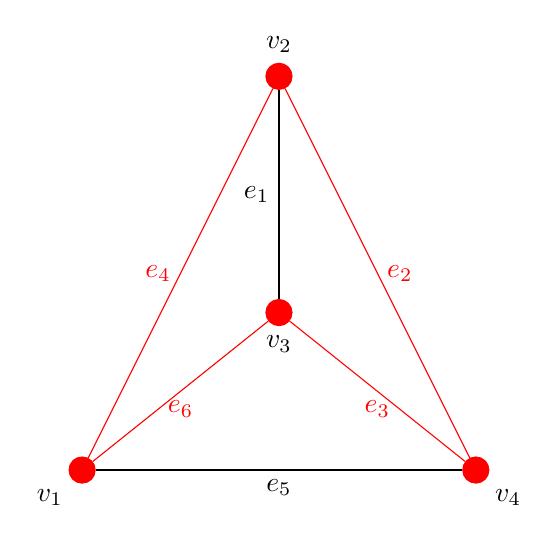
\begin{tikzpicture}
    
                \node[shape=circle, draw=red, fill=red, label=below left:$v_1$] (A) at (-2.5,-2) {};
                \node[shape=circle, draw=red, fill=red, label=above:$v_2$] (B) at (0,3) {};
                \node[shape=circle, draw=red, fill=red, label=below:$v_3$] (C) at (0,0) {};
                \node[shape=circle, draw=red, fill=red, label=below right:$v_4$] (D) at (2.5,-2) {};
            
                \draw (C) -- (B) node[midway, left] {$e_1$};
                \draw[red] (B) -- (D) node[midway, right] {$e_2$};
                \draw[red] (D) -- (C) node[midway, below] {$e_3$};
                \draw[red] (A) -- (B) node[midway, left] {$e_4$};
                \draw (D) -- (A) node[midway, below] {$e_5$};
                \draw[red] (A) -- (C) node[midway, below] {$e_6$};
        
            \end{tikzpicture}
            
        \end{center}

    \end{frame}

    \begin{frame}{Cycles}

        \begin{center}
        
            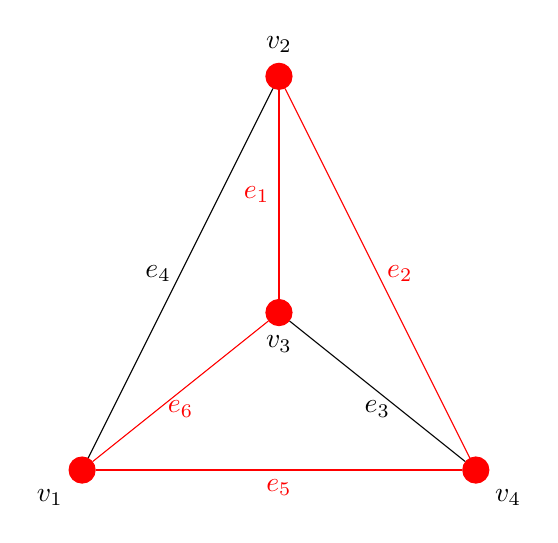
\begin{tikzpicture}
    
                \node[shape=circle, draw=red, fill=red, label=below left:$v_1$] (A) at (-2.5,-2) {};
                \node[shape=circle, draw=red, fill=red, label=above:$v_2$] (B) at (0,3) {};
                \node[shape=circle, draw=red, fill=red, label=below:$v_3$] (C) at (0,0) {};
                \node[shape=circle, draw=red, fill=red, label=below right:$v_4$] (D) at (2.5,-2) {};
            
                \draw[red] (C) -- (B) node[midway, left] {$e_1$};
                \draw[red] (B) -- (D) node[midway, right] {$e_2$};
                \draw (D) -- (C) node[midway, below] {$e_3$};
                \draw (A) -- (B) node[midway, left] {$e_4$};
                \draw[red] (D) -- (A) node[midway, below] {$e_5$};
                \draw[red] (A) -- (C) node[midway, below] {$e_6$};
        
            \end{tikzpicture}
            
        \end{center}

    \end{frame}

    \begin{frame}{Cycle Bases}

        A \textbf{spanning tree} is a subset $T\subseteq E$ which meets every vertex but contains no cycles.

        \vspace{12pt}

        A \textbf{cycle basis} is a set of cycles which cover every edge (and are linearly independent) -- these only exist for 2-connected graphs.

        \vspace{12pt}
        
        One can be found by considering the \textbf{fundamental cycles} with respect to a spanning tree.

    \end{frame}

    \begin{frame}{Cycle Bases}

        \begin{center}
        
            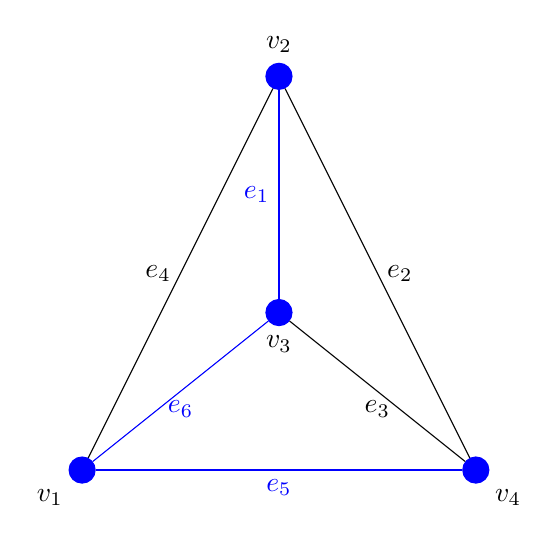
\begin{tikzpicture}
    
                \node[shape=circle, draw=blue, fill=blue, label=below left:$v_1$] (A) at (-2.5,-2) {};
                \node[shape=circle, draw=blue, fill=blue, label=above:$v_2$] (B) at (0,3) {};
                \node[shape=circle, draw=blue, fill=blue, label=below:$v_3$] (C) at (0,0) {};
                \node[shape=circle, draw=blue, fill=blue, label=below right:$v_4$] (D) at (2.5,-2) {};
            
                \draw[blue] (C) -- (B) node[midway, left] {$e_1$};
                \draw (B) -- (D) node[midway, right] {$e_2$};
                \draw (D) -- (C) node[midway, below] {$e_3$};
                \draw (A) -- (B) node[midway, left] {$e_4$};
                \draw[blue] (D) -- (A) node[midway, below] {$e_5$};
                \draw[blue] (A) -- (C) node[midway, below] {$e_6$};
        
            \end{tikzpicture}

            \vspace{-12pt}

            \textcolor{white}{\[C_1=\{e_1, e_4, e_6\}, C_2=\{e_1, e_2, e_5, e_6\}, C_3=\{e_3, e_5, e_6\}\]}
            
        \end{center}

    \end{frame}

    \begin{frame}{Cycle Bases}

        \begin{center}
        
            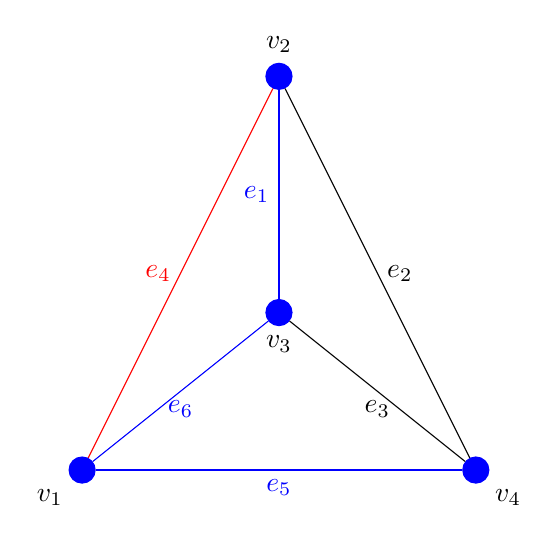
\begin{tikzpicture}
    
                \node[shape=circle, draw=blue, fill=blue, label=below left:$v_1$] (A) at (-2.5,-2) {};
                \node[shape=circle, draw=blue, fill=blue, label=above:$v_2$] (B) at (0,3) {};
                \node[shape=circle, draw=blue, fill=blue, label=below:$v_3$] (C) at (0,0) {};
                \node[shape=circle, draw=blue, fill=blue, label=below right:$v_4$] (D) at (2.5,-2) {};
            
                \draw[blue] (C) -- (B) node[midway, left] {$e_1$};
                \draw (B) -- (D) node[midway, right] {$e_2$};
                \draw (D) -- (C) node[midway, below] {$e_3$};
                \draw[red] (A) -- (B) node[midway, left] {$e_4$};
                \draw[blue] (D) -- (A) node[midway, below] {$e_5$};
                \draw[blue] (A) -- (C) node[midway, below] {$e_6$};
        
            \end{tikzpicture}

            \vspace{-12pt}

            \textcolor{white}{\[C_1=\{e_1, e_4, e_6\}, C_2=\{e_1, e_2, e_5, e_6\}, C_3=\{e_3, e_5, e_6\}\]}
            
        \end{center}

    \end{frame}

    \begin{frame}{Cycle Bases}

        \begin{center}
        
            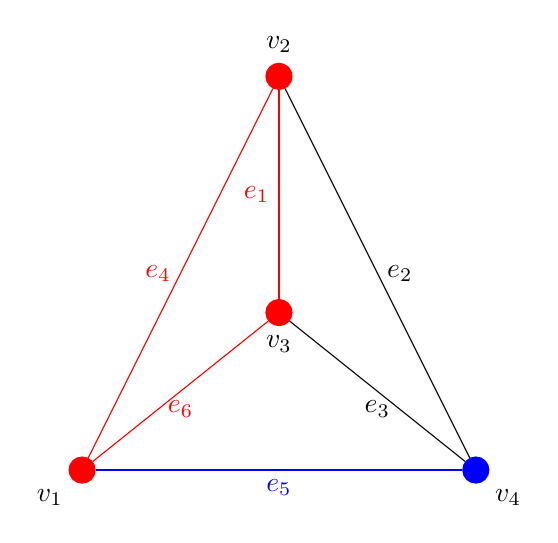
\begin{tikzpicture}
    
                \node[shape=circle, draw=red, fill=red, label=below left:$v_1$] (A) at (-2.5,-2) {};
                \node[shape=circle, draw=red, fill=red, label=above:$v_2$] (B) at (0,3) {};
                \node[shape=circle, draw=red, fill=red, label=below:$v_3$] (C) at (0,0) {};
                \node[shape=circle, draw=blue, fill=blue, label=below right:$v_4$] (D) at (2.5,-2) {};
            
                \draw[red] (C) -- (B) node[midway, left] {$e_1$};
                \draw (B) -- (D) node[midway, right] {$e_2$};
                \draw (D) -- (C) node[midway, below] {$e_3$};
                \draw[red] (A) -- (B) node[midway, left] {$e_4$};
                \draw[blue] (D) -- (A) node[midway, below] {$e_5$};
                \draw[red] (A) -- (C) node[midway, below] {$e_6$};
        
            \end{tikzpicture}

            \[C_1=\{e_1, e_4, e_6\}\textcolor{white}{, C_2=\{e_1, e_2, e_5, e_6\}, C_3=\{e_3, e_5, e_6\}}\]
            
        \end{center}

    \end{frame}

    \begin{frame}{Cycle Bases}

        \begin{center}
        
            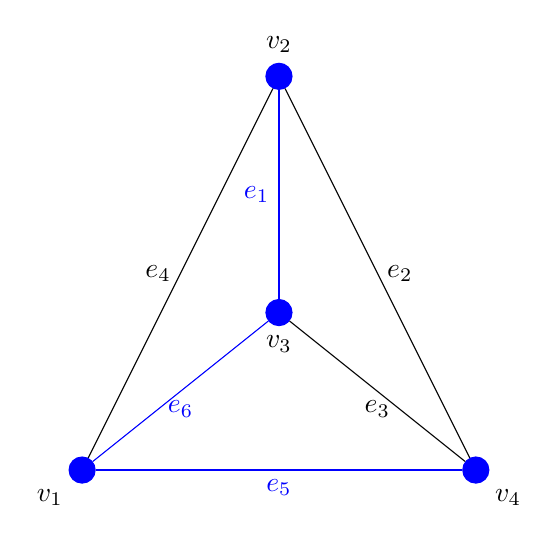
\begin{tikzpicture}
    
                \node[shape=circle, draw=blue, fill=blue, label=below left:$v_1$] (A) at (-2.5,-2) {};
                \node[shape=circle, draw=blue, fill=blue, label=above:$v_2$] (B) at (0,3) {};
                \node[shape=circle, draw=blue, fill=blue, label=below:$v_3$] (C) at (0,0) {};
                \node[shape=circle, draw=blue, fill=blue, label=below right:$v_4$] (D) at (2.5,-2) {};
            
                \draw[blue] (C) -- (B) node[midway, left] {$e_1$};
                \draw (B) -- (D) node[midway, right] {$e_2$};
                \draw (D) -- (C) node[midway, below] {$e_3$};
                \draw (A) -- (B) node[midway, left] {$e_4$};
                \draw[blue] (D) -- (A) node[midway, below] {$e_5$};
                \draw[blue] (A) -- (C) node[midway, below] {$e_6$};
        
            \end{tikzpicture}

            \[C_1=\{e_1, e_4, e_6\}\textcolor{white}{, C_2=\{e_1, e_2, e_5, e_6\}, C_3=\{e_3, e_5, e_6\}}\]
            
        \end{center}

    \end{frame}

    \begin{frame}{Cycle Bases}

        \begin{center}
        
            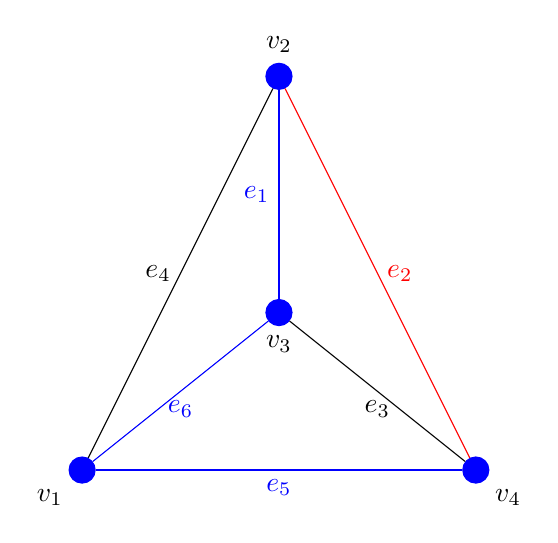
\begin{tikzpicture}
    
                \node[shape=circle, draw=blue, fill=blue, label=below left:$v_1$] (A) at (-2.5,-2) {};
                \node[shape=circle, draw=blue, fill=blue, label=above:$v_2$] (B) at (0,3) {};
                \node[shape=circle, draw=blue, fill=blue, label=below:$v_3$] (C) at (0,0) {};
                \node[shape=circle, draw=blue, fill=blue, label=below right:$v_4$] (D) at (2.5,-2) {};
            
                \draw[blue] (C) -- (B) node[midway, left] {$e_1$};
                \draw[red] (B) -- (D) node[midway, right] {$e_2$};
                \draw (D) -- (C) node[midway, below] {$e_3$};
                \draw (A) -- (B) node[midway, left] {$e_4$};
                \draw[blue] (D) -- (A) node[midway, below] {$e_5$};
                \draw[blue] (A) -- (C) node[midway, below] {$e_6$};
        
            \end{tikzpicture}

            \[C_1=\{e_1, e_4, e_6\}\textcolor{white}{, C_2=\{e_1, e_2, e_5, e_6\}, C_3=\{e_3, e_5, e_6\}}\]
            
        \end{center}

    \end{frame}

    \begin{frame}{Cycle Bases}

        \begin{center}
        
            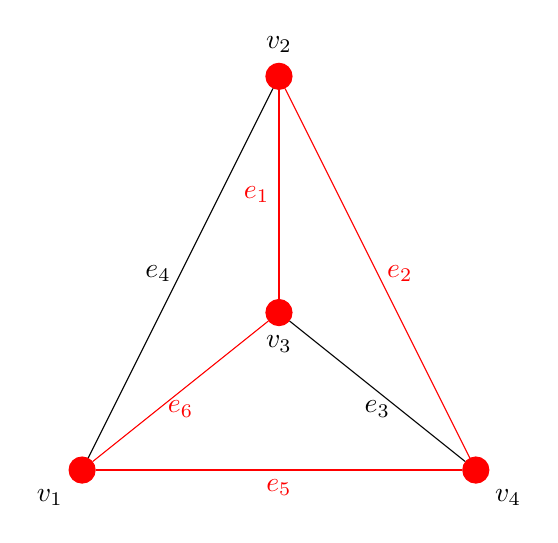
\begin{tikzpicture}
    
                \node[shape=circle, draw=red, fill=red, label=below left:$v_1$] (A) at (-2.5,-2) {};
                \node[shape=circle, draw=red, fill=red, label=above:$v_2$] (B) at (0,3) {};
                \node[shape=circle, draw=red, fill=red, label=below:$v_3$] (C) at (0,0) {};
                \node[shape=circle, draw=red, fill=red, label=below right:$v_4$] (D) at (2.5,-2) {};
            
                \draw[red] (C) -- (B) node[midway, left] {$e_1$};
                \draw[red] (B) -- (D) node[midway, right] {$e_2$};
                \draw (D) -- (C) node[midway, below] {$e_3$};
                \draw (A) -- (B) node[midway, left] {$e_4$};
                \draw[red] (D) -- (A) node[midway, below] {$e_5$};
                \draw[red] (A) -- (C) node[midway, below] {$e_6$};
        
            \end{tikzpicture}

            \[C_1=\{e_1, e_4, e_6\}, C_2=\{e_1, e_2, e_5, e_6\}\textcolor{white}{, C_3=\{e_3, e_5, e_6\}}\]
            
        \end{center}

    \end{frame}

    \begin{frame}{Cycle Bases}

        \begin{center}
        
            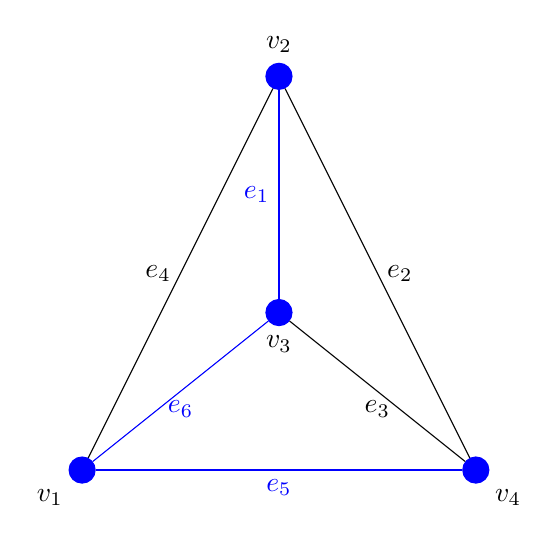
\begin{tikzpicture}
    
                \node[shape=circle, draw=blue, fill=blue, label=below left:$v_1$] (A) at (-2.5,-2) {};
                \node[shape=circle, draw=blue, fill=blue, label=above:$v_2$] (B) at (0,3) {};
                \node[shape=circle, draw=blue, fill=blue, label=below:$v_3$] (C) at (0,0) {};
                \node[shape=circle, draw=blue, fill=blue, label=below right:$v_4$] (D) at (2.5,-2) {};
            
                \draw[blue] (C) -- (B) node[midway, left] {$e_1$};
                \draw (B) -- (D) node[midway, right] {$e_2$};
                \draw (D) -- (C) node[midway, below] {$e_3$};
                \draw (A) -- (B) node[midway, left] {$e_4$};
                \draw[blue] (D) -- (A) node[midway, below] {$e_5$};
                \draw[blue] (A) -- (C) node[midway, below] {$e_6$};
        
            \end{tikzpicture}

            \[C_1=\{e_1, e_4, e_6\}, C_2=\{e_1, e_2, e_5, e_6\}\textcolor{white}{, C_3=\{e_3, e_5, e_6\}}\]
            
        \end{center}

    \end{frame}

    \begin{frame}{Cycle Bases}

        \begin{center}
        
            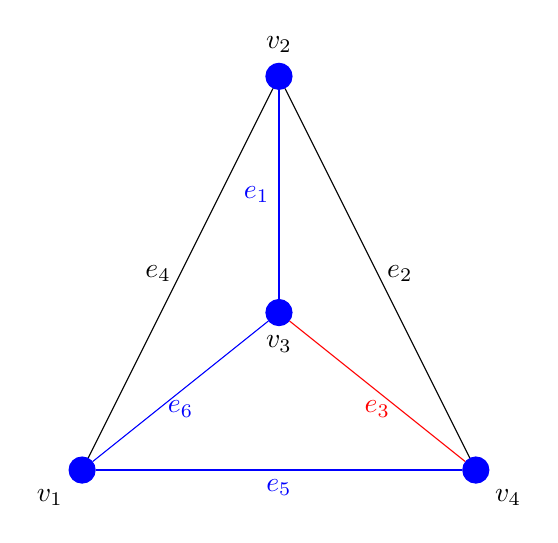
\begin{tikzpicture}
    
                \node[shape=circle, draw=blue, fill=blue, label=below left:$v_1$] (A) at (-2.5,-2) {};
                \node[shape=circle, draw=blue, fill=blue, label=above:$v_2$] (B) at (0,3) {};
                \node[shape=circle, draw=blue, fill=blue, label=below:$v_3$] (C) at (0,0) {};
                \node[shape=circle, draw=blue, fill=blue, label=below right:$v_4$] (D) at (2.5,-2) {};
            
                \draw[blue] (C) -- (B) node[midway, left] {$e_1$};
                \draw (B) -- (D) node[midway, right] {$e_2$};
                \draw[red] (D) -- (C) node[midway, below] {$e_3$};
                \draw (A) -- (B) node[midway, left] {$e_4$};
                \draw[blue] (D) -- (A) node[midway, below] {$e_5$};
                \draw[blue] (A) -- (C) node[midway, below] {$e_6$};
        
            \end{tikzpicture}

            \[C_1=\{e_1, e_4, e_6\}, C_2=\{e_1, e_2, e_5, e_6\}\textcolor{white}{, C_3=\{e_3, e_5, e_6\}}\]
            
        \end{center}

    \end{frame}

    \begin{frame}{Cycle Bases}

        \begin{center}
        
            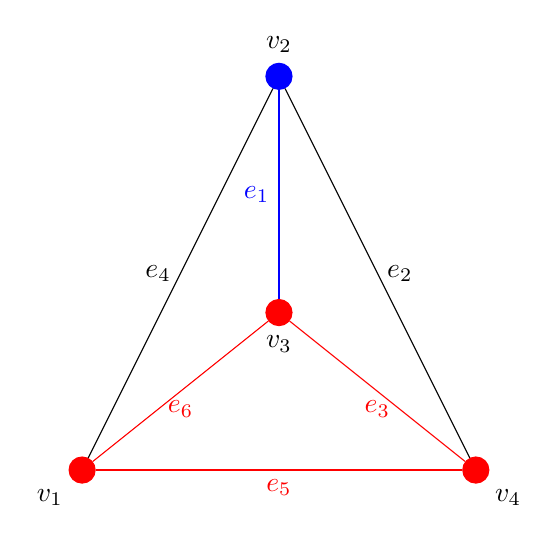
\begin{tikzpicture}
    
                \node[shape=circle, draw=red, fill=red, label=below left:$v_1$] (A) at (-2.5,-2) {};
                \node[shape=circle, draw=blue, fill=blue, label=above:$v_2$] (B) at (0,3) {};
                \node[shape=circle, draw=red, fill=red, label=below:$v_3$] (C) at (0,0) {};
                \node[shape=circle, draw=red, fill=red, label=below right:$v_4$] (D) at (2.5,-2) {};
            
                \draw[blue] (C) -- (B) node[midway, left] {$e_1$};
                \draw (B) -- (D) node[midway, right] {$e_2$};
                \draw[red] (D) -- (C) node[midway, below] {$e_3$};
                \draw (A) -- (B) node[midway, left] {$e_4$};
                \draw[red] (D) -- (A) node[midway, below] {$e_5$};
                \draw[red] (A) -- (C) node[midway, below] {$e_6$};
        
            \end{tikzpicture}

            \[C_1=\{e_1, e_4, e_6\}, C_2=\{e_1, e_2, e_5, e_6\}, C_3=\{e_3, e_5, e_6\}.\]
            
        \end{center}

    \end{frame}

    \begin{frame}{Oriented Cycle Bases}

        An orientation on a graph causes cycles to become \textbf{oriented cycles}.

        \vspace{12pt}

        Start following an edge clockwise (or counterclockwise), if an edges orientation agrees along the cycle it gets a positive coefficient, otherwise negative.

        \vspace{12pt}

        We call a cycle \textbf{positive} (or \textbf{negative}) if the coefficients are all positive (or negative).

        \vspace{12pt}
        
        A \textbf{positive cycle basis} consists of positive cycles.

    \end{frame}

    \begin{frame}{Oriented Cycle Bases}

        \begin{center}
        
            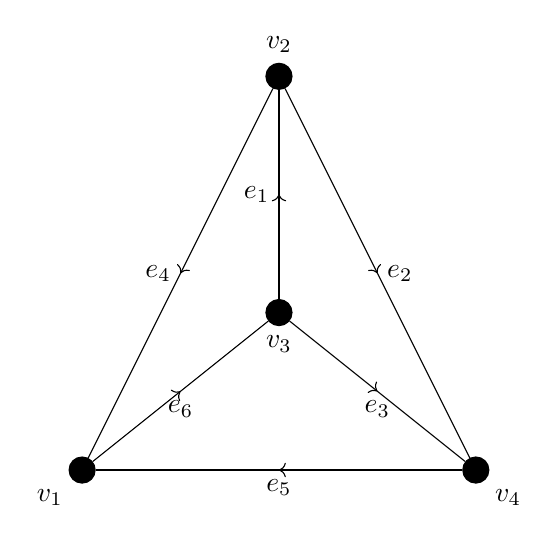
\begin{tikzpicture}
            
                \node[shape=circle, draw=black, fill=black, label=below left:$v_1$] (A) at (-2.5,-2) {};
                \node[shape=circle, draw=black, fill=black, label=above:$v_2$] (B) at (0,3) {};
                \node[shape=circle, draw=black, fill=black, label=below:$v_3$] (C) at (0,0) {};
                \node[shape=circle, draw=black, fill=black, label=below right:$v_4$] (D) at (2.5,-2) {};
            
                \draw[->-] (C) -- (B) node[midway, left] {$e_1$};
                \draw[->-] (B) -- (D) node[midway, right] {$e_2$};
                \draw[->-] (C) -- (D) node[midway, below] {$e_3$};
                \draw[->-] (B) -- (A) node[midway, left] {$e_4$};
                \draw[->-] (D) -- (A) node[midway, below] {$e_5$};
                \draw[->-] (A) -- (C) node[midway, below] {$e_6$};
        
            \end{tikzpicture}

            \[C_1=\{+e_1, +e_4, +e_6\}, C_2=\{+e_1, +e_2, +e_5, +e_6\}, C_3=\{+e_3, +e_5, +e_6\}.\]
            
        \end{center}

    \end{frame}

    \begin{frame}{Dual (Planar) Graph}

        \begin{center}
    
            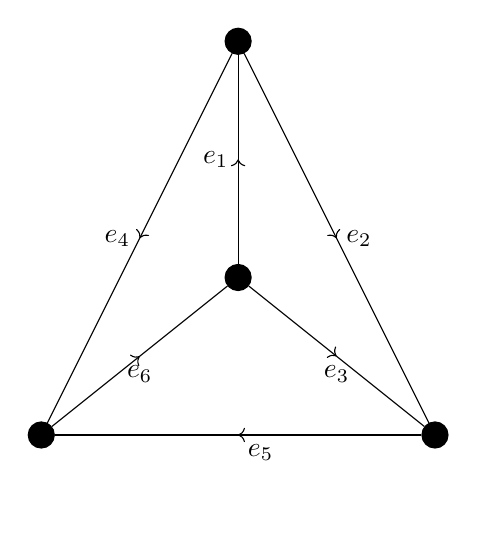
\begin{tikzpicture}
            
                \node[shape=circle, draw=black, fill=black] (A) at (-2.5,-2) {};
                \node[shape=circle, draw=black, fill=black] (B) at (0,3) {};
                \node[shape=circle, draw=black, fill=black] (C) at (0,0) {};
                \node[shape=circle, draw=black, fill=black] (D) at (2.5,-2) {};
                \node[shape=circle, draw=white, fill=white] (H) at (0,-3) {};
            
                \draw[->-] (C) -- (B) node[midway, left] {$e_1$};
                \draw[->-] (B) -- (D) node[midway, right] {$e_2$};
                \draw[->-] (C) -- (D) node[midway, below] {$e_3$};
                \draw[->-] (B) -- (A) node[midway, left] {$e_4$};
                \draw[->-] (D) -- (A) node[midway, below right] {$e_5$};
                \draw[->-] (A) -- (C) node[midway, below] {$e_6$};
        
            \end{tikzpicture}
        
        \end{center}
        
    \end{frame}

    \begin{frame}{Dual (Planar) Graph}

        \begin{center}
    
            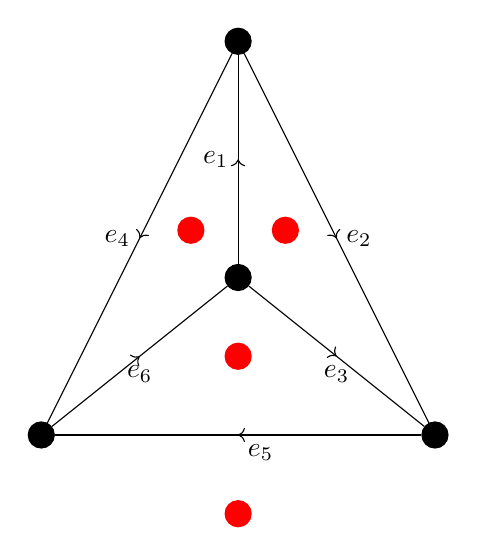
\begin{tikzpicture}
            
                \node[shape=circle, draw=black, fill=black] (A) at (-2.5,-2) {};
                \node[shape=circle, draw=black, fill=black] (B) at (0,3) {};
                \node[shape=circle, draw=black, fill=black] (C) at (0,0) {};
                \node[shape=circle, draw=black, fill=black] (D) at (2.5,-2) {};
                \node[shape=circle, draw=red, fill=red] (E) at (-0.6,0.6) {};
                \node[shape=circle, draw=red, fill=red] (F) at (0.6,0.6) {};
                \node[shape=circle, draw=red, fill=red] (G) at (0,-1) {};
                \node[shape=circle, draw=red, fill=red] (H) at (0,-3) {};
            
                \draw[->-] (C) -- (B) node[midway, left] {$e_1$};
                \draw[->-] (B) -- (D) node[midway, right] {$e_2$};
                \draw[->-] (C) -- (D) node[midway, below] {$e_3$};
                \draw[->-] (B) -- (A) node[midway, left] {$e_4$};
                \draw[->-] (D) -- (A) node[midway, below right] {$e_5$};
                \draw[->-] (A) -- (C) node[midway, below] {$e_6$};
        
            \end{tikzpicture}
        
        \end{center}
        
    \end{frame}

    \begin{frame}{Dual (Planar) Graph}

        \begin{center}
    
            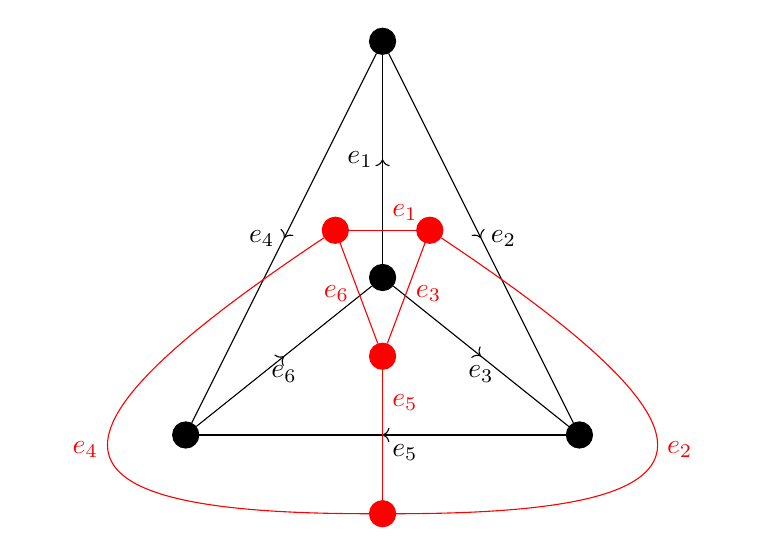
\begin{tikzpicture}
            
                \node[shape=circle, draw=black, fill=black] (A) at (-2.5,-2) {};
                \node[shape=circle, draw=black, fill=black] (B) at (0,3) {};
                \node[shape=circle, draw=black, fill=black] (C) at (0,0) {};
                \node[shape=circle, draw=black, fill=black] (D) at (2.5,-2) {};
                \node[shape=circle, draw=red, fill=red] (E) at (-0.6,0.6) {};
                \node[shape=circle, draw=red, fill=red] (F) at (0.6,0.6) {};
                \node[shape=circle, draw=red, fill=red] (G) at (0,-1) {};
                \node[shape=circle, draw=red, fill=red] (H) at (0,-3) {};
            
                \draw[->-] (C) -- (B) node[midway, left] {$e_1$};
                \draw[->-] (B) -- (D) node[midway, right] {$e_2$};
                \draw[->-] (C) -- (D) node[midway, below] {$e_3$};
                \draw[->-] (B) -- (A) node[midway, left] {$e_4$};
                \draw[->-] (D) -- (A) node[midway, below right] {$e_5$};
                \draw[->-] (A) -- (C) node[midway, below] {$e_6$};
                \draw[red] (E) -- (F) node[midway, above right, red] {$e_1$};
                \draw[red] (H) .. controls (4.5, -3) and (4.5, -2) .. (F) node[midway, right, red] {$e_2$};
                \draw[red] (F) -- (G) node[midway, right, red] {$e_3$};
                \draw[red] (E) .. controls (-4.5, -2) and (-4.5, -3) .. (H) node[midway, left, red] {$e_4$};
                \draw[red] (H) -- (G) node[near end, right, red] {$e_5$};
                \draw[red] (E) -- (G) node[midway, left, red] {$e_6$};
        
            \end{tikzpicture}
        
        \end{center}
        
    \end{frame}

    \begin{frame}{Dual (Planar) Graph}

        \begin{center}
    
            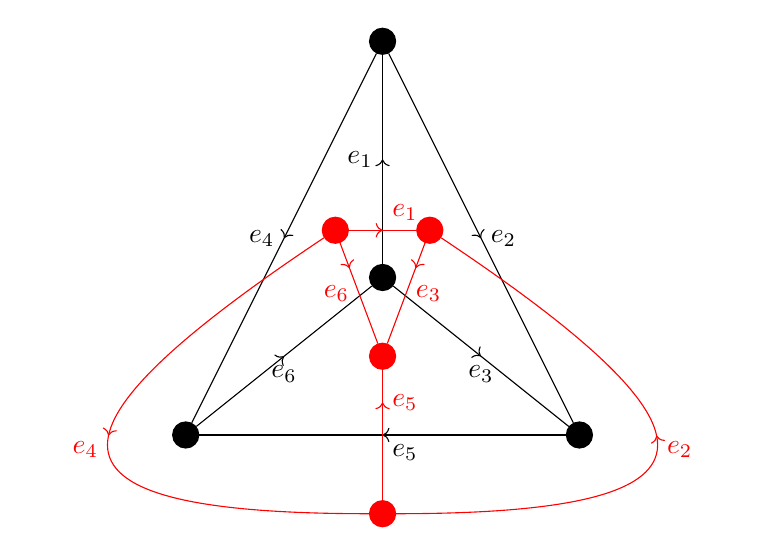
\begin{tikzpicture}
            
                \node[shape=circle, draw=black, fill=black] (A) at (-2.5,-2) {};
                \node[shape=circle, draw=black, fill=black] (B) at (0,3) {};
                \node[shape=circle, draw=black, fill=black] (C) at (0,0) {};
                \node[shape=circle, draw=black, fill=black] (D) at (2.5,-2) {};
                \node[shape=circle, draw=red, fill=red] (E) at (-0.6,0.6) {};
                \node[shape=circle, draw=red, fill=red] (F) at (0.6,0.6) {};
                \node[shape=circle, draw=red, fill=red] (G) at (0,-1) {};
                \node[shape=circle, draw=red, fill=red] (H) at (0,-3) {};
            
                \draw[->-] (C) -- (B) node[midway, left] {$e_1$};
                \draw[->-] (B) -- (D) node[midway, right] {$e_2$};
                \draw[->-] (C) -- (D) node[midway, below] {$e_3$};
                \draw[->-] (B) -- (A) node[midway, left] {$e_4$};
                \draw[->-] (D) -- (A) node[midway, below right] {$e_5$};
                \draw[->-] (A) -- (C) node[midway, below] {$e_6$};
                \draw[->-, red] (E) -- (F) node[midway, above right, red] {$e_1$};
                \draw[->-, red] (H) .. controls (4.5, -3) and (4.5, -2) .. (F) node[midway, right, red] {$e_2$};
                \draw[->--, red] (F) -- (G) node[midway, right, red] {$e_3$};
                \draw[->-, red] (E) .. controls (-4.5, -2) and (-4.5, -3) .. (H) node[midway, left, red] {$e_4$};
                \draw[-->-, red] (H) -- (G) node[near end, right, red] {$e_5$};
                \draw[->--, red] (E) -- (G) node[midway, left, red] {$e_6$};
        
            \end{tikzpicture}
        
        \end{center}
        
    \end{frame}

    \begin{frame}{The Lattice of Integer Flows -- Graphs}

        Considering $\Z^E$ to be the free abelian group spanned by $E(G)$, the \textbf{lattice of integer flows} of a graph is the abelian subgroup of $\Z^E$ spanned by cycles, equipped with the Euclidean inner product.

        \pause

        \vspace{12pt}
        
        Any cycle basis then is a basis of the lattice of integer flows.

        \pause

        \vspace{12pt}

        The \textit{discrete Torelli theorem} for a certain class of objects states that their lattices of integer flows are isomorphic iff the objects are.

        \pause

        \vspace{12pt}

        \begin{itemize}
            \item Graphs -- Watkins (1990, 1994)\pause
            \item Graphs and tropical curves -- Caporaso and Viviani (2010)\pause
            \item Regular matroids -- Su and Wagner (2010)
        \end{itemize}
        
    \end{frame}

    \begin{frame}{Matroid}

        A matroid is a formalism which generalises graphs and linear algebra -- we consider trees independent and cycles dependent.
        
        \pause

        \vspace{12pt}

        A (finite) \textbf{matroid} $\calM=(E, \calI)$ is an ordered pair of a finite set $E$, called the \textbf{base set}, and $\calI$, called the ``family of independent subsets of $E$" which satisfies the following axioms:
        
        \begin{enumerate}
    
            \item $\emptyset\in\calI$.
            \item  For any $I_1\in\calI$ and $I_2\subseteq I_1$, then $I_2\in\calI$.
            \item If $I_1, I_2\in\calI$ are such that $\abs*{I_1}<\abs*{I_2}$, then there exists $e\in I_2\setminus I_1$ such that $I_1\cup\{e\}\in\calI$.
            
        \end{enumerate}

        \pause

        \vspace{12pt}
    
        \begin{itemize}
            \item \textbf{Dependent sets} are those which are not independent, denoted $\calD$.\pause
            \item \textbf{Circuit sets} are minimal dependent sets, denoted $\calC$.\pause
            \item \textbf{Basis sets} are maximal independent sets, denoted $\calB$.\pause
        \end{itemize}

        \vspace{12pt}

        Any of the above can define a matroid, they each come with a set of axioms.

    \end{frame}

    \begin{frame}{Motivating Examples of Matroids}

        \begin{enumerate}
            \item Given a matrix $M$ over $\mathbb{F}$, letting $E(\calM)$ be the columns of $M$, then a matroid is formed in the natural way of linear independence.
            Such a matroid is called a \textbf{$\mathbb{F}$-representable matroid}.\pause
            \item Given a graph $G$, letting $E(\calM)=E(G)$ and $\calC(\calM)$ consist of the cycles in $G$, then $\calM(G)$ is the \textbf{graphical matroid associated to $G$}.
            Note vertices do not exist in graphical matroids!\pause
        \end{enumerate}

        A matroid which is representable over any field is called a \textbf{regular matroid}.
        Any graphical matroid is regular by finding the graphs signed adjacency matrix.
        
    \end{frame}

    \begin{frame}{Regular Matroids}

        Regular matroids are nice -- very similar to graphs.
        Many notions transfer over:\pause

        \begin{itemize}
            \item Spanning trees $\rightarrow$ basis sets.\pause
            \item Cycle bases $\rightarrow$ circuit bases.\pause
            \item $2$-connected graph $\rightarrow$ cogirth $\geq2$ matroid (every $e\in E$ is in some cycle).\pause
            \item Orientations (edge assignments) $\rightarrow$ orientations (column assignments).\pause
            \item Strongly connected orientations: path between vertices $\rightarrow$ every $e\in E$ is in a positive circuit.\pause
            \item Dual graph (only planar) $\rightarrow$ dual matroid -- works for non-planar!\pause
            \item Induced dual orientation $\rightarrow$ oriented dual matroid.\pause
        \end{itemize}
        In fact regular matroids are closed under duality, and graphical matroids and their duals (almost) generate all regular matroids.
        
    \end{frame}

    \begin{frame}{The Lattice of Integer Flows -- Matroids}
        
        Given a regular matroid $\calM$ with representing matrix $M$, the lattice of integer flows is

        \[\calF(\calM)=\ker(M)\cap\Z^E.\]
        This coincides for the signed incidence matrix of a graph -- the natural representing matrix for a graphical matroid.

        \vspace{12pt}
        
        Any circuit basis then is a basis of the lattice of integer flows.
        
    \end{frame}

    \begin{frame}{Recovering $\calM$}

        The lattice of integer flows is a (in most cases strict) sub-lattice of $\Z^E$.
        Can we explicitly recover $\calM$ from $\calF(\calM)$?

        \pause

        \vspace{12pt}

        We provide a constructive algorithm for recovering the matroid -- a \textit{constructive Torelli theorem}.
        The first step is strengthening the following theorem.

        \vspace{12pt}

        \theorem{[Su-Wagner] Let $\calM$ and $\calN$ be 2-connected regular matroids.
        Then $\calF(\calM)\cong\calF(\calN)$ if and only if $\calM\cong\calN$.}

        \pause

        \vspace{12pt}
        
        \proposition{A positive circuit basis exists for any 2-connected regular matroid.}

    \end{frame}

    \begin{frame}{Lifting Isomorphisms}

        \proposition{An isomorphism of lattices $\varphi:\calF(\calM)\rightarrow\calF(\calN)$ lifts to an isomorphism of Euclidean lattices $\Phi:\Z^{E(\calM)}\rightarrow\Z^{E(\calN)}$.}\pause

        \vspace{12pt}

        \proof

        \begin{enumerate}
            \item Use Greene's rigid embedding theorem to show any automorphism of $\calF(\calM)$ lifts -- relies on the existance of a positive circuit basis of $\calM$.\pause
            \item
        \end{enumerate}

        \begin{center}

            \begin{tikzcd}[row sep=large,column sep=huge,ampersand replacement=\&]
                \textcolor{white}{\Z^{E(\calM)}}
                    \arrow[white]{r}[white]{\Psi}
                \& \Z^{E(\calN)}
                    
                \& \Z^{E(\calM)}
                    \arrow[dashed]{l}[swap]{\Phi}
                    \arrow[bend right, white]{ll}[swap, white]{F}
                    \\
                \textcolor{white}{\calF(\calM)}
                    \arrow[white]{r}[swap, white]{\psi}
                    \arrow[hookrightarrow, white]{u}[white]{}
                \& \calF(\calN)
                    \arrow[hookrightarrow, white]{u}[swap, white]{}
                \& \calF(\calM)
                    \arrow{l}{\varphi}
                    \arrow[hookrightarrow, white]{u}[swap, white]{}
                    \arrow[bend left, white]{ll}[white]{\psi^{-1}\circ\varphi}

            \end{tikzcd}
            
        \end{center}
        
    \end{frame}

    \begin{frame}{Lifting Isomorphisms}

        \proposition{An isomorphism of lattices $\varphi:\calF(\calM)\rightarrow\calF(\calN)$ lifts to an isomorphism of Euclidean lattices $\Phi:\Z^{E(\calM)}\rightarrow\Z^{E(\calN)}$.}

        \vspace{12pt}

        \proof

        \begin{enumerate}
            \item Use Greene's rigid embedding theorem to show any automorphism of $\calF(\calM)$ lifts -- relies on the existance of a positive circuit basis of $\calM$.
            \item
        \end{enumerate}

        \begin{center}

            \begin{tikzcd}[row sep=large,column sep=huge,ampersand replacement=\&]
                \Z^{E(\calM)}
                    \arrow{r}{\Psi}
                \& \Z^{E(\calN)}
                    
                \& \Z^{E(\calM)}
                    \arrow[dashed]{l}[swap]{\Phi}
                    \arrow[bend right, white]{ll}[swap, white]{F}
                    \\
                \textcolor{white}{\calF(\calM)}
                    \arrow[white]{r}[swap, white]{\psi}
                    \arrow[hookrightarrow, white]{u}[white]{}
                \& \calF(\calN)
                    \arrow[hookrightarrow, white]{u}[swap, white]{}
                \& \calF(\calM)
                    \arrow{l}{\varphi}
                    \arrow[hookrightarrow, white]{u}[swap, white]{}
                    \arrow[bend left, white]{ll}[white]{\psi^{-1}\circ\varphi}

            \end{tikzcd}
            
        \end{center}
        
    \end{frame}

    \begin{frame}{Lifting Isomorphisms}

        \proposition{An isomorphism of lattices $\varphi:\calF(\calM)\rightarrow\calF(\calN)$ lifts to an isomorphism of Euclidean lattices $\Phi:\Z^{E(\calM)}\rightarrow\Z^{E(\calN)}$.}

        \vspace{12pt}

        \proof

        \begin{enumerate}
            \item Use Greene's rigid embedding theorem to show any automorphism of $\calF(\calM)$ lifts -- relies on the existance of a positive circuit basis of $\calM$.
            \item
        \end{enumerate}

        \begin{center}

            \begin{tikzcd}[row sep=large,column sep=huge,ampersand replacement=\&]
                \Z^{E(\calM)}
                    \arrow{r}{\Psi}
                \& \Z^{E(\calN)}
                    
                \& \Z^{E(\calM)}
                    \arrow[dashed]{l}[swap]{\Phi}
                    \arrow[bend right, white]{ll}[swap, white]{F}
                    \\
                \calF(\calM)
                    \arrow{r}[swap]{\psi}
                    \arrow[hookrightarrow, white]{u}[white]{}
                \& \calF(\calN)
                    \arrow[hookrightarrow, white]{u}[swap, white]{}
                \& \calF(\calM)
                    \arrow{l}{\varphi}
                    \arrow[hookrightarrow, white]{u}[swap, white]{}
                    \arrow[bend left, white]{ll}[white]{\psi^{-1}\circ\varphi}
            \end{tikzcd}
            
        \end{center}
        
    \end{frame}

    \begin{frame}{Lifting Isomorphisms}

        \proposition{An isomorphism of lattices $\varphi:\calF(\calM)\rightarrow\calF(\calN)$ lifts to an isomorphism of Euclidean lattices $\Phi:\Z^{E(\calM)}\rightarrow\Z^{E(\calN)}$.}

        \vspace{12pt}

        \proof

        \begin{enumerate}
            \item Use Greene's rigid embedding theorem to show any automorphism of $\calF(\calM)$ lifts -- relies on the existance of a positive circuit basis of $\calM$.
            \item
        \end{enumerate}

        \begin{center}

            \begin{tikzcd}[row sep=large,column sep=huge,ampersand replacement=\&]
                \Z^{E(\calM)}
                    \arrow{r}{\Psi}
                \& \Z^{E(\calN)}
                    
                \& \Z^{E(\calM)}
                    \arrow[dashed]{l}[swap]{\Phi}
                    \arrow[bend right, white]{ll}[swap, white]{F}
                    \\
                \calF(\calM)
                    \arrow{r}[swap]{\psi}
                    \arrow[hookrightarrow, white]{u}[white]{}
                \& \calF(\calN)
                    \arrow[hookrightarrow, white]{u}[swap, white]{}
                \& \calF(\calM)
                    \arrow{l}{\varphi}
                    \arrow[hookrightarrow, white]{u}[swap, white]{}
                    \arrow[bend left]{ll}{\psi^{-1}\circ\varphi}
            \end{tikzcd}
            
        \end{center}
        
    \end{frame}

    \begin{frame}{Lifting Isomorphisms}

        \proposition{An isomorphism of lattices $\varphi:\calF(\calM)\rightarrow\calF(\calN)$ lifts to an isomorphism of Euclidean lattices $\Phi:\Z^{E(\calM)}\rightarrow\Z^{E(\calN)}$.}

        \vspace{12pt}

        \proof

        \begin{enumerate}
            \item Use Greene's rigid embedding theorem to show any automorphism of $\calF(\calM)$ lifts -- relies on the existance of a positive circuit basis of $\calM$.
            \item
        \end{enumerate}

        \begin{center}

            \begin{tikzcd}[row sep=large,column sep=huge,ampersand replacement=\&]
                \Z^{E(\calM)}
                    \arrow{r}{\Psi}
                \& \Z^{E(\calN)}
                    
                \& \Z^{E(\calM)}
                    \arrow[dashed]{l}[swap]{\Phi}
                    \arrow[bend right]{ll}[swap]{F}
                    \\
                \calF(\calM)
                    \arrow{r}[swap]{\psi}
                    \arrow[hookrightarrow, white]{u}[white]{}
                \& \calF(\calN)
                    \arrow[hookrightarrow, white]{u}[swap, white]{}
                \& \calF(\calM)
                    \arrow{l}{\varphi}
                    \arrow[hookrightarrow, white]{u}[swap, white]{}
                    \arrow[bend left]{ll}{\psi^{-1}\circ\varphi}
            \end{tikzcd}
            
        \end{center}
        
    \end{frame}

    \begin{frame}{Lifting Isomorphisms}

        \proposition{An isomorphism of lattices $\varphi:\calF(\calM)\rightarrow\calF(\calN)$ lifts to an isomorphism of Euclidean lattices $\Phi:\Z^{E(\calM)}\rightarrow\Z^{E(\calN)}$.}

        \vspace{12pt}

        \proof

        \begin{enumerate}
            \item Use Greene's rigid embedding theorem to show any automorphism of $\calF(\calM)$ lifts -- relies on the existance of a positive circuit basis of $\calM$.
            \item
        \end{enumerate}

        \begin{center}

            \begin{tikzcd}[row sep=large,column sep=huge,ampersand replacement=\&]
                \Z^{E(\calM)}
                    \arrow{r}{\Psi}
                \& \Z^{E(\calN)}
                    
                \& \Z^{E(\calM)}
                    \arrow[dashed]{l}[swap]{\Phi:=\Psi\circ F}
                    \arrow[bend right]{ll}[swap]{F}
                    \\
                \calF(\calM)
                    \arrow{r}[swap]{\psi}
                    \arrow[hookrightarrow]{u}{}
                \& \calF(\calN)
                    \arrow[hookrightarrow]{u}[swap]{}
                \& \calF(\calM)
                    \arrow{l}{\varphi}
                    \arrow[hookrightarrow]{u}[swap]{}
                    \arrow[bend left]{ll}{\psi^{-1}\circ\varphi}
            \end{tikzcd}
            
        \end{center}

        \hspace*{\fill}\qedsymbol
        
    \end{frame}

    \begin{frame}{Voronoi Cells}

        The \textbf{Voronoi cell} $\calV(\Lambda)$ of a lattice $\Lambda$ is the collection of points in space (i.e. in $\Lambda\otimes\mathbb{R}$) closer to the origin than any other lattice point in $\Lambda$.

        \pause

    \begin{center}
        
            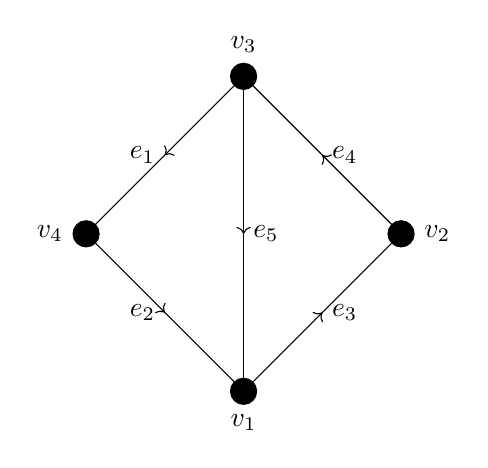
\begin{tikzpicture}
            
                \node[shape=circle, draw=black, fill=black, label=below:$v_1$] (A) at (0,0) {};
                \node[shape=circle, draw=black, fill=black, label=right:$v_2$] (B) at (2,2) {};
                \node[shape=circle, draw=black, fill=black, label=above:$v_3$] (C) at (0,4) {};
                \node[shape=circle, draw=black, fill=black, label=left:$v_4$] (D) at (-2,2) {};
            
                \draw[->-] (C) -- (D) node[midway, left] {$e_1$};
                \draw[->-] (D) -- (A) node[midway, left] {$e_2$};
                \draw[->-] (A) -- (B) node[midway, right] {$e_3$};
                \draw[->-] (B) -- (C) node[midway, right] {$e_4$};
                \draw[->-] (C) -- (A) node[midway, right] {$e_5$};
        
            \end{tikzpicture}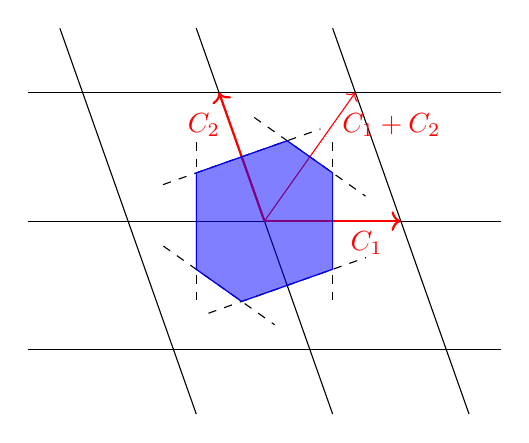
\begin{tikzpicture}

                %sqrt3=1.73205081
                %1/sqrt3=0.57735027
                %2sqrt2/sqrt3=1.63299316
                %1/2sqrt2=0.35355339
                %sqrt2=1.41421356

                \draw (-3,-1.63299316) -- (3,-1.63299316);
                \draw (-3,0) -- (3,0);
                \draw (-3,1.63299316) -- (3,1.63299316);
                \draw (-0.57735027*1.5-1.73205081,1.63299316*1.5) -- (0.57735027*1.5-1.73205081,-1.63299316*1.5);
                \draw (-0.57735027*1.5,1.63299316*1.5) -- (0.57735027*1.5,-1.63299316*1.5);
                \draw (-0.57735027*1.5+1.73205081,1.63299316*1.5) -- (0.57735027*1.5+1.73205081,-1.63299316*1.5);

                \draw[dashed, name path=line 1] (-1.73205081/2,1) -- (-1.73205081/2,-1);
                \draw[dashed, name path=line 2] (1.73205081/2,1) -- (1.73205081/2,-1);
                \draw[dashed, name path=line 3] (-0.57735027/2-1,1.63299316/2-0.35355339) -- (-0.57735027/2+1,1.63299316/2+0.35355339);
                \draw[dashed, name path=line 4] (0.57735027/2-1,-1.63299316/2-0.35355339) -- (0.57735027/2+1,-1.63299316/2+0.35355339);
                \draw[dashed, name path=line 5] (-0.57735027/2+1.73205081/2-1.41421356*1/2,1.63299316/2+1/2) -- (-0.57735027/2+1.73205081/2+1.41421356*1/2,1.63299316/2-1/2);
                \draw[dashed, name path=line 6] (0.57735027/2-1.73205081/2-1.41421356*1/2,-1.63299316/2+1/2) -- (0.57735027/2-1.73205081/2+1.41421356*1/2,-1.63299316/2-1/2);

                \draw[->, thick, red] (0,0) -- (1.73205081,0) node[near end, below, red] {$C_1$};
                \draw[->, thick, red] (0,0) -- (-0.57735027,1.63299316) node[near end, left, red] {$C_2$};
                \draw[->, red] (0,0) -- (-0.57735027+1.73205081,1.63299316) node[near end, right, red] {$C_1+C_2$};

                \path[name intersections={of=line 1 and line 3, by=A}];
                \path[name intersections={of=line 1 and line 6, by=B}];
                \path[name intersections={of=line 4 and line 6, by=C}];
                \path[name intersections={of=line 2 and line 4, by=D}];
                \path[name intersections={of=line 2 and line 5, by=E}];
                \path[name intersections={of=line 3 and line 5, by=F}];

                \draw[fill=blue, opacity=0.5] (A) -- (B) -- (C) -- (D) -- (E) -- (F) -- (A);

                \def\points{(A), (B), (C), (D), (E), (F), (A)}
                
                \foreach \p [count=\i, remember=\p as \lastp] in \points{
                    \ifnum\i>1\relax
                    %\node[shape=circle, scale=0.2, draw=blue, fill=blue]  at \p {};
                    \path[draw=blue, fill=blue] \lastp -- \p;
                    \fi
                }

            \end{tikzpicture}

            \[C_1=\{+e_1, +e_2, -e_5\}, C_2=\{+e_3, +e_4, +e_5\}, C_1+C_2=\{+e_1, +e_2, +e_3, +e_4\}.\]
        
        \end{center}
        
    \end{frame}

    \begin{frame}{Amini-Dancso-Lim Theorem}

        Faces of the Voronoi cell form a partially ordered set (poset) $\calF\calP(\calF(\calM))$ with inclusion given by dimension.

        \vspace{12pt}

        Oriented submatroids $(\calM, \omega_\calM)$ which are strongly connected form a poset $\calS\calC(\calM)$ with inclusion $(\calM, \omega_\calM)\leq(\calN, \omega_\calN)$ if and only if $\calN$ is a submatroid of $\calM$ and $\omega_\calM$ restricted to $\calN$ is $\omega_\calN$.

        \vspace{12pt}

        \theorem{For a finite regular matroid $\calM$, $\calF\calP(\calF(\calM))\cong\calS\calC(\calM)$ as graded posets.}

        \vspace{12pt}

        \example{Codimension one faces of the Voronoi cell correspond to circuits in $\calM$.
        Edges of the Voronoi cell correspond to maximal strongly orientable submatroids of $\calM$.}
        
    \end{frame}

    \begin{frame}{Amini-Dancso-Lim Theorem}

        The parallel faces of the Voronoi cell correspond to the different strongly connected orientations of the same underlying matroid.

        \vspace{12pt}
        
        For a face $F$, we consider $[F]$ the \textbf{equivalence class of faces that are parallel to $F$}.

        \vspace{12pt}

        For a subset $A\subseteq E(\calM)$ we denote $[F_A]$ to be the face(s) which corresponds to $\calM\setminus A$ (provided it is strongly orientable).
        
    \end{frame}

    \begin{frame}{Reconstruction for 3-connected Matroids}

        A matroid is 3-connected if $\calM\setminus\{e\}$ is 2-connected for all $e\in E(\calM)$.
        Furthermore, a 2-connected matroid can always be strongly oriented as it always has a positive circuit basis.

        \vspace{12pt}

        Reconstructing 3-connected matroids:

        \pause

        \begin{enumerate}
            \item There is a bijection $e\leftrightarrow [F_{\{e\}}]$ for $e\in E(\calM)$.\pause
            \item There is a bijection $C\leftrightarrow [F_C]$ for $C\in\calC(\calM)$.\pause
            \item A given element $e\in E(\calM)$ belongs to a circuit $C$ if and only if no member of $[F_{\{e\}}]$ is contained in $[F_C]$.\pause
        \end{enumerate}

        \vspace{12pt}

        For general 2-connected matroids steps (2) and (3) remain the same, but step (1) requires much more work, as maximal strongly connected submatroids may be of the form $\calM\setminus S$ for (possibly different sized) $\abs*{S}>1$.
        
    \end{frame}

    \begin{frame}{Reconstruction for 2-connected Matroids}

        The key to the reconstruction for 2-connected matroids are \textbf{2-cut blocks}.

        \vspace{12pt}
        
        These are the equivalence classes of the equivalence relation $e\sim f$ if and only if $e=f$ or $\{e, f\}$ is a cocircuit (a circuit in the dual matroid).

        \vspace{12pt}
        
        These 2-cut blocks are precisely those sets for which $\calM\setminus S$ is a maximal strongly connected submatroid, so denote $S_{[\epsilon]}$ for the 2-cut block which corresponds to the parallel class of edges $[\epsilon]$.

    \end{frame}

    \begin{frame}{Reconstruction for 2-connected Matroids}
        
        \begin{enumerate}
            \item Create a circuit basis $B$ such that $\abs*{\iprod*{C_i, C_j}}=\abs*{C_i\cap C_j}$ for all $C_i, C_j\in B$.\pause
            \item Find the parallel classes $[\epsilon]$ of the Voronoi cell and identify which edges participate in $F_C$ for each $C\in B$.\pause
            \item For each basis circuit $C_i, i=1, \dots, r$, write the equation

            \[\sum_{[\epsilon]\not\in F_{C_i}} \abs*{S_{[\epsilon]}}=\iprod*{C_i, C_i},\]
            and for each pair of basis circuits $\{\{C_i, C_j\}, i, j=1, \dots, r, i\neq j\}$ write the equation
            
            \[\sum_{[\epsilon]\not\in F_{C_i}, F_{C_j}} \abs*{S_{[\epsilon]}}=\abs*{\iprod*{C_i, C_j}}.\]\pause
            \item Find the unique positive integer solution $\{\abs*{S_{[\epsilon]}}\}$.\pause
            \item $E(\calM)$ is the disjoint union of the sets $\{S_{[\epsilon]}\}$.\pause
            \item Again, the element $e$ belongs to a circuit $C$ if and only if no member of the corresponding edge parallel class $[\epsilon]$ belongs to the face $[F_C]$.
        \end{enumerate}
        
    \end{frame}

    \begin{frame}{Reconstructing}

        \begin{minipage}{0.4\textwidth}

            \begin{figure}[htbp]
            
                \begin{center}
            
                    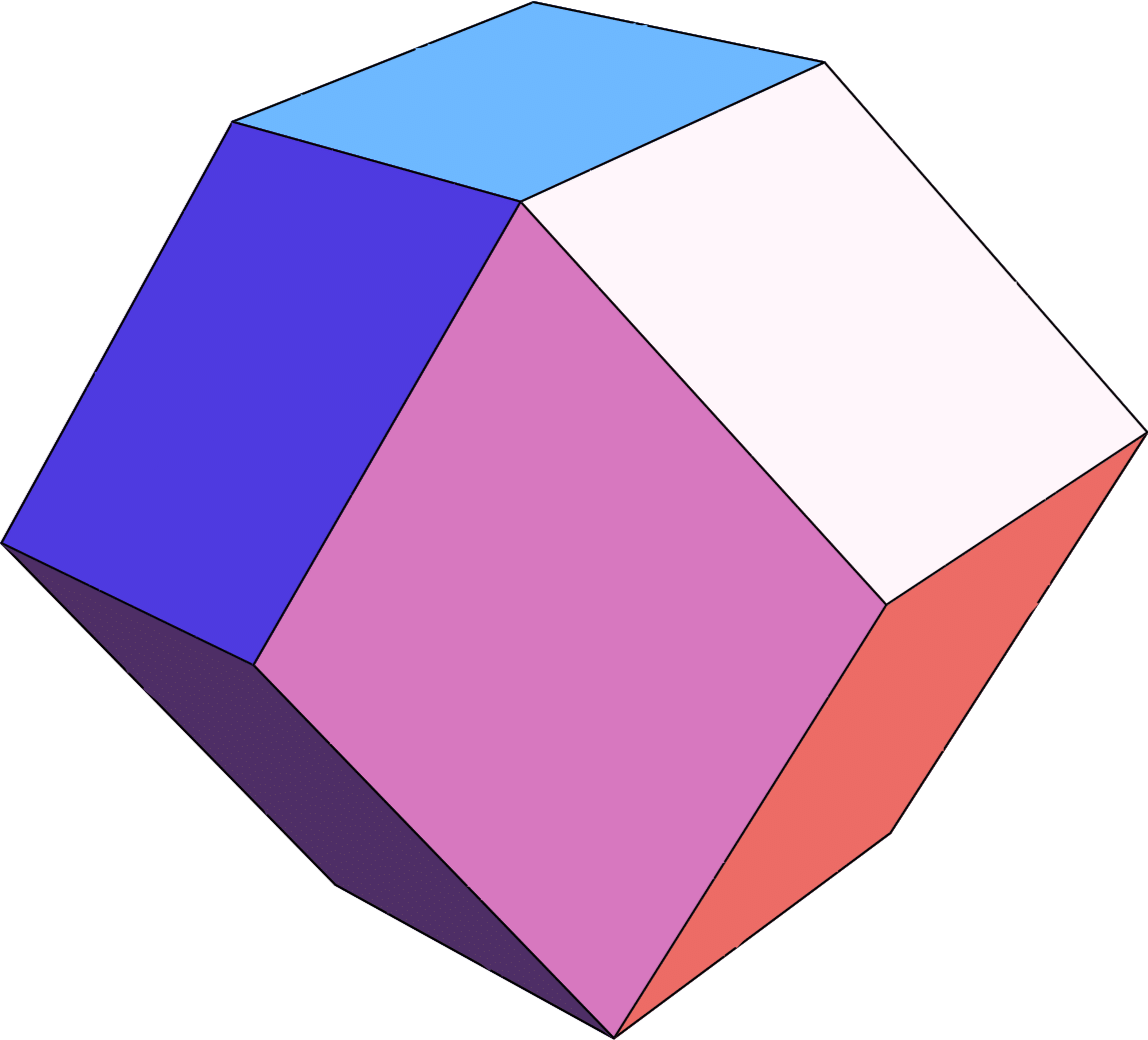
\includegraphics[height=3cm]{RhombicDodecahedron.png}
                    
                \end{center}
                
            \end{figure}

            \[\begin{blockarray}{cccc}
                & C_1 & C_2 & C_3\\
                \begin{block}{c(ccc)}
                    C_1 & 3 & 1 & 2\\
                    C_2 & 1 & 3 & 0\\
                    C_3 & 2 & 0 & 4\\
                \end{block}
            \end{blockarray}\]
            
        \end{minipage}\resizebox{0.1\textwidth}{!}{$\rightarrow$}\begin{minipage}{0.5\textwidth}

            \begin{figure}[htbp]
            
                \begin{center}
    
                    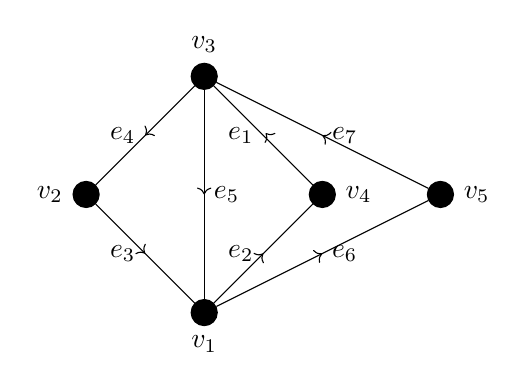
\begin{tikzpicture}[scale=0.75]
                    
                        \node[shape=circle, draw=black, fill=black, label=below:$v_1$] (A) at (0,0) {};
                        \node[shape=circle, draw=black, fill=black, label=left:$v_2$] (B) at (-2,2) {};
                        \node[shape=circle, draw=black, fill=black, label=above:$v_3$] (C) at (0,4) {};
                        \node[shape=circle, draw=black, fill=black, label=right:$v_4$] (D) at (2,2) {};
                        \node[shape=circle, draw=black, fill=black, label=right:$v_5$] (E) at (4,2) {};
                    
                        \draw[->-] (D) -- (C) node[midway, left] {$e_1$};
                        \draw[->-] (A) -- (D) node[midway, left] {$e_2$};
                        \draw[->-] (B) -- (A) node[midway, left] {$e_3$};
                        \draw[->-] (C) -- (B) node[midway, left] {$e_4$};
                        \draw[->-] (C) -- (A) node[midway, right] {$e_5$};
                        \draw[->-] (A) -- (E) node[midway, right] {$e_6$};
                        \draw[->-] (E) -- (C) node[midway, right] {$e_7$};
                
                    \end{tikzpicture}
                
                \end{center}
            
            \end{figure}

            \vspace{-24pt}

            \begin{align*}
                C_1&=\{+e_1, +e_2, +e_5\},\\
                C_2&=\{+e_5, +e_6, +e_7\},\\
                C_3&=\{+e_1, +e_2, +e_3, +e_4\}.
            \end{align*}

        \end{minipage}
        
    \end{frame}

    \begin{frame}{Greene's Conjecture}

        Greene showed that:

        \vspace{12pt}

        \theorem{The $d$-invariant of the lattice of integer flows of a 2-connected graph determines its stable isomorphism type.}
        
        \vspace{12pt}

        Then naturally conjectured:

        \vspace{12pt}

        \conjecture{The $d$-invariant of the lattice of integer flows of a 2-connected regular matroid determines its stable isomorphism type.}

        \vspace{12pt}

        The approach we used shows most of what is required for this conjecture to be true.
        
    \end{frame}
    
\end{document}